\chapter{Introduction}
\label{chap:intro}

\section{Research Background}
\label{sec:research-background}

Three-dimensional (3D) rendering is the computationally intensive process of generating photorealistic images from geometric scene descriptions, a cornerstone technology in film production, video game development, architectural visualisation, and interactive media. A single high-fidelity frame may require hours of computation on a dedicated workstation; rendering a full animation sequence at production quality demands thousands of such frames~\cite{christensen2016path}. The consequent demand for computational power has driven the 3D rendering industry towards cloud GPU platforms, where rendering studios rent time on GPU nodes rather than maintaining on-premise hardware infrastructure.

Cloud GPU markets have matured rapidly. Platforms such as RunPod, Lambda Labs, and CoreWeave now offer heterogeneous GPU fleets (comprising nodes with different architectures, memory capacities, and performance profiles) at a range of price points~\cite{runpod2026podspricing,coreweave2026pricing,lambda2026pricing}, with billing granularity as fine as one second on RunPod~\cite{runpod2026podspricing}. A rendering studio submitting jobs to such a platform faces a multi-dimensional optimisation challenge: jobs arrive stochastically, GPU node availability fluctuates due to competing customers, maintenance windows, and hardware failures, and jobs carry soft or hard deadlines tied to production schedules. Selecting the wrong GPU for a job, or failing to schedule deadline-critical frames promptly, can cascade into missed delivery milestones and financial penalties.

Scheduling in heterogeneous cloud computing environments has been an active research area since the early~2000s~\cite{braun2001comparison,topcuoglu2002heft}. However, the specific combination of features present in cloud GPU rendering (per-second billing, qualitative rather than exact node availability information, stochastic provisioning delays driven by competing customer demand, and real-world GPU performance heterogeneity at the rendering-task level) has, to the best of the author's knowledge, not been studied as a unified problem. Existing surveys on GPU scheduling in data centres~\cite{ye2024deep} focus primarily on deep learning training workloads, where the access model (reserved clusters or dedicated hardware) differs fundamentally from the marketplace rental model used in cloud rendering.

This study addresses this gap by formulating the \textbf{Cloud GPU Rendering Scheduling Problem (CGRSP)}: a mathematical model and empirical evaluation framework for scheduling 3D rendering workloads on heterogeneous, stochastically available GPU fleets. At its core, CGRSP asks: \emph{given a stream of rendering jobs arriving over time, one job per frame, each with a deadline, a complexity level, and an estimated execution duration, and given a heterogeneous fleet of GPU nodes with stochastic availability, which GPU should each job be assigned to, and in what order should jobs be processed, to jointly minimise waiting time, deadline miss rate, and operational cost?}

Three challenges make CGRSP hard in practice:

\begin{enumerate}

\item \textbf{GPU Heterogeneity.} The fleet in this study consists of four GPU types (RTX~3090, RTX~A5000, RTX~A4000, and RTX~A4500) with differing CUDA core counts, VRAM capacities, per-hour rental prices, and empirical rendering speeds. A simple rule such as ``assign the fastest GPU'' maximises throughput but ignores cost; ``assign the cheapest GPU'' minimises cost but may increase waiting time and deadline violations. The optimal assignment depends on the job's complexity, deadline urgency, and the current fleet state.

\item \textbf{Stochastic Node Availability.} In a public cloud GPU market, a studio cannot guarantee that a GPU of the required type can be acquired promptly when a job needs it. Customer demand fluctuates diurnally, maintenance windows are scheduled by the platform, and hardware failures occur with non-zero probability, all of which shrink the rentable pool. The simulator models this as a stochastic, stock-status-dependent provisioning delay at acquisition (on the on-demand Secure Cloud pool studied here, a held instance is never reclaimed mid-job), and the scheduler observes only a coarsened state abstraction (idle / running, plus per-type stock status), reflecting what is actually visible to a cloud consumer through a platform API.

\item \textbf{Bi-Objective Optimisation.} Rendering studios care about both \emph{turnaround time} (minimising the time a job waits before execution begins) and \emph{cost} (minimising the total GPU rental fees). These objectives are in partial tension: GPU types differ in both execution time and rental rate, and their performance ranking can change with job complexity (fleet pricing in Table~\ref{tab:gpu_specs}). A scheduler must navigate this trade-off explicitly.

\end{enumerate}

Figure~\ref{fig:problem-overview} sketches the end-to-end problem: rendering jobs arrive stochastically and queue for capacity; at each event a scheduler decides which job runs on which GPU; the heterogeneous fleet executes the work; and each job's outcome is recorded as its waiting time, deadline adherence, and rental cost. The three challenges above map directly onto this flow: heterogeneity lives in the fleet, stochastic availability sits between the scheduler and the fleet, and the bi-objective tension appears in the outcomes.

\begin{figure}[htbp]
\centering
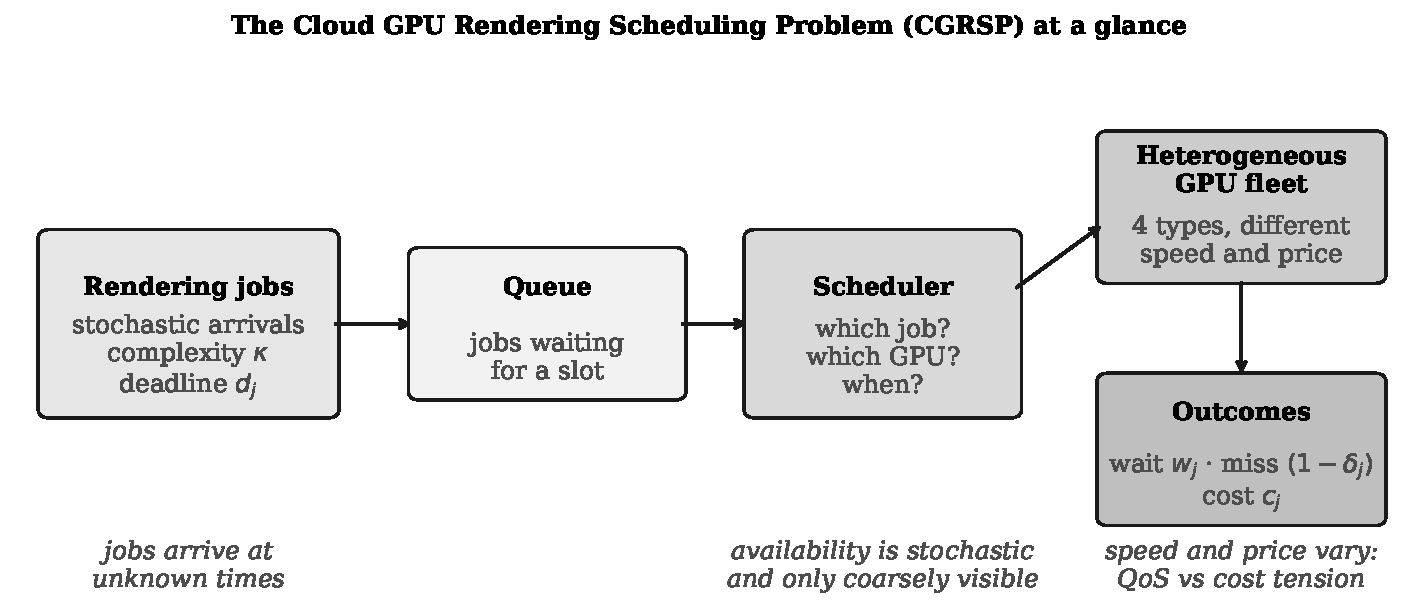
\includegraphics[width=0.97\textwidth]{figures/problem_overview.pdf}
\caption[The CGRSP problem at a glance]{The Cloud GPU Rendering Scheduling Problem at a glance. Rendering jobs with a complexity level and a deadline arrive stochastically and wait in a queue; the scheduler decides which job to place on which GPU and when; the heterogeneous fleet (four GPU types with different speeds and prices, and stochastic availability) executes the jobs; and per-job outcomes (waiting time, deadline adherence, cost) are the quantities the scheduler is judged on.}
\label{fig:problem-overview}
\end{figure}

The formulation is grounded in 6,234 real rendering jobs logged by the author's RunPod rendering pipeline (6,030 from its production Serverless endpoint, 203 tagged as development runs and one with no environment tag) and is evaluated through a discrete-event simulator calibrated to March 2026 RunPod pricing.

\section{Computational Complexity}
\label{sec:computational-complexity}

The offline version of CGRSP (where all $n$ jobs are known in advance) is a generalisation of the weighted job scheduling problem on parallel unrelated machines with deadlines, which is NP-hard in the strong sense~\cite{pinedo2016scheduling}. For the online version (jobs revealed at their arrival times), online deadline-constrained scheduling without preemption admits no general worst-case performance guarantee against the offline optimum; even on a single preemptive processor, deadline-driven scheduling is optimal only while the system is underloaded~\cite{liu1973scheduling,dertouzos1974control}, and under overload no online algorithm can guarantee more than one quarter of the value achievable with full knowledge of future arrivals~\cite{baruah1992competitiveness}. This intractability motivates the use of practical heuristic policies rather than exact optimisation. The heuristic policies are benchmarked in Chapter~\ref{chap:experiments} against a FIFO baseline, with a certified capacity bound and a clairvoyant relaxation as additional reference points, rather than against an intractable optimum; reinforcement learning is a natural future extension (Section~\ref{sec:limitations-and-future-research}) but is not evaluated in this study.

\section{Research Objective}
\label{sec:research-objective}

This study pursues four research objectives:

\begin{enumerate}

\item \textbf{Formal Problem Formulation.} Define CGRSP as a rigorous mathematical optimisation problem with explicit notation, decision variables, constraints, and a bi-objective function, enabling reproducible comparison with future work.

\item \textbf{Simulator Construction and Calibration.} Build a discrete-event simulator of an on-demand RunPod Secure Cloud fleet, including empirically measured GPU execution times, a stochastic availability model, Poisson job arrivals, and per-second cost tracking, with its service-time inputs calibrated to 6,234 real rendering jobs and its schedules checked by a constraint verifier.

\item \textbf{Comparative Evaluation of Scheduling Heuristics.} Implement and statistically compare ten scheduling algorithms: FIFO (baseline), Shortest Processing Time (SPT), Earliest Deadline First (EDF), Lowest Cost First (LCF), Balanced (weighted speed-cost composite), Random, SPT+Rescue (SPT with laxity-based deadline rescue), an adaptive queue-pressure EDF-SPT hybrid, the novel anticipative Rolling-Horizon (RH) scheduler, and the Cost-Aware Deadline-Risk (CADR) scheduler. Assess them across a four-phase evaluation programme: single-seed benchmark, 30-seed statistical validation, day-type and deadline-tightness sensitivity, and a 30-day monthly simulation whose day-type mix is taken from real RunPod billing data.

\item \textbf{Deployment Guidance.} Translate experimental findings into actionable recommendations, grounded in paired statistical tests, for cloud rendering operators: establish which of the two proposed schedulers should be the default and when the other is preferable (CADR as the default, since its paired baseline miss difference from RH is not significant (equivalence untested), it has close monthly miss point estimates with lower tardiness, and it leads under eased availability and the data-ordered per-type ranking; RH as the specialist for the scarce baseline availability regime when only the count of missed deadlines matters, and SPT for operators who prioritise queue wait), quantify when SPT's wait-time advantage outweighs its deadline risk, identify the tight-deadline fraction threshold at which EDF becomes preferable, and characterise the role of the concurrency limit $C_{\max}$ as the primary performance lever.

\end{enumerate}

\section{Research Contribution}
\label{sec:research-contribution}

The primary contributions of this study are:

\begin{itemize}

\item A complete mathematical formulation of CGRSP, including a three-state availability model (its unavailable state is retained for generality and does not occur on the on-demand platform studied), a bi-objective QoS-cost function, and all assignment and temporal constraints (Chapter~\ref{chap:formulation}).

\item A verified discrete-event simulator implemented in Python, calibrated against the full empirical rendering-job dataset (Chapter~\ref{chap:system}).

\item A statistically rigorous comparison of ten scheduling algorithms (eight benchmarks, including an adaptive EDF-SPT hybrid, plus the two proposed schedulers) on the saturated hectic-day configuration of Section~\ref{ssec:platform-and-data} ($n=30$ seeds, $\rho>1$), using paired $t$-tests, Cohen's $d$ effect sizes, and a Holm-Bonferroni correction. The comparison establishes SPT as the lowest-wait baseline (with no significant paired wait difference from RH), but significantly outperformed by EDF on miss, and quantifies the deadline penalty of the deadline-oblivious policies (Chapter~\ref{chap:experiments}).

\item A day-type sensitivity study (quiet/normal/hectic/surge, 30 seeds each) showing that the scheduler ranking is regime-dependent: RH has the lowest miss point estimate on hectic days (above saturation, $\rho>1$; no significant paired miss difference from CADR in the Phase~3 30-seed test), while the Adaptive hybrid, EDF, and RH form the lowest miss tier on below-saturation surge days (no paired test is computed for the day-type sweep) (Chapter~\ref{chap:experiments}).

\item A deadline-tightness sensitivity study under the surge-day configuration of Section~\ref{ssec:platform-and-data} (30 seeds per sweep point) locating the crossover between deadline-driven and shortest-job-first ordering: among the seven baseline policies in the sweep, EDF attains significantly lower miss than SPT when tight fraction $\leq 30\%$, the paired test does not resolve their difference at the midpoint of the sweep ($50\%$), and SPT attains significantly lower miss from $\geq 70\%$; no scheduler achieves 0\% misses across all fractions at surge-day load (Chapter~\ref{chap:experiments}).

\item A 30-day monthly operational simulation (Phase~4, 10 replications) whose mix of day types is taken from RunPod billing data (22~April to 21~May 2026), showing that RH and CADR remain the lowest-miss pair at monthly scale (near-identical, RH marginally lower, with no paired test at that phase), while RH's hectic-day wait advantage does not carry over, and identifying the concurrency budget $C_{\max}$ as the binding throughput constraint at the assumed hectic-day stress load (Chapter~\ref{chap:experiments}).

\item Two complementary deadline-aware schedulers: (i) the Rolling-Horizon (RH) scheduler, which at each event plans over the slot-availability timeline and anticipated arrivals, keeping shortest-processing-time ordering for jobs with slack, promoting only jobs the timeline shows would otherwise miss, and demoting jobs projected to miss under mean-service estimates to prioritise jobs projected to meet their deadlines; RH has the lowest deadline miss point estimate of the ten policies (no significant paired difference from CADR in Phase~3) with no significant paired wait difference from SPT, significantly outperforming SPT+Rescue on miss; and (ii) the Cost-Aware Deadline-Risk (CADR) scheduler, which classifies jobs by a scale-free critical ratio and selects the cheapest deadline-feasible node; CADR has a close miss point estimate to RH at substantially lower tardiness, has close monthly miss point estimates with lower tardiness, and leads under eased availability and the data-ordered per-type ranking, and also has a lower miss point estimate than SPT+Rescue (no pre-specified paired test), at essentially the same wait. The study recommends CADR as the default scheduler and RH as the specialist for the scarce baseline availability regime when only the miss count matters; operators who prioritise queue wait should use SPT (Chapter~\ref{chap:experiments}; see also Research Objective~4 above).

\end{itemize}

\section{Scope and Limitations}
\label{sec:scope-and-limitations}

This study focuses on scheduling 3D rendering workloads in a simulated on-demand GPU fleet modelled with RunPod Secure Cloud prices from March 2026. The evaluation is based on the empirical dataset of real rendering jobs collected between July 2025 and June 2026, spanning four GPU types (RTX~3090, RTX~A5000, RTX~A4000, RTX~A4500) and three scene complexity levels.

Several limitations bound the scope of this work. The baseline concurrency limit is five instances, RunPod's default per-account worker quota ($C_{\max}$, Section~\ref{ssec:platform-and-data}), which serves as the primary throughput constraint and is varied only in a dedicated sensitivity sweep. The hectic and surge workloads are stress loads above the busiest recorded day, and operating costs use RunPod Pods (Secure Cloud) prices although the job data came from a Serverless endpoint. The baseline availability probabilities are modelling assumptions rather than measured frequencies, since the author's pricing-API snapshots show the fleet types almost never at High stock and often with no Secure Cloud offer at all; a sensitivity sweep over the assumed baseline availability probabilities (Chapter~\ref{chap:experiments}) shows that the proposed and rescue-style deadline-aware policies stay ahead of the deadline-blind ones at every operable setting (plain EDF ties SPT at the scarcer $\times0.75$ setting), but the order within the leading pair is not stable: RH's miss lead over CADR is significant only at the scarcer operable setting, the most eased setting lets several policies reach zero misses while RH does not, and permuting the per-type ranking to the order the snapshot record's offer shares support moves the lead to CADR; the scarcest settings leave the fleet inoperable for every policy alike (Chapter~\ref{chap:conclusion}). The study also assumes non-preemptive scheduling, as CGRSP models each rendering frame as a single indivisible job and does not split a frame into pixels, samples, tiles or sub-frames; rendering one frame across multiple GPUs is not considered. A six-mix fleet-composition sweep at ten seeds is a sensitivity check on one workload, not a second studio trace, and the learned baseline in the comparison is a shallow tabular bandit rather than a deep policy, so its null result is not evidence about deep reinforcement learning. These limitations are discussed in detail, together with directions for future research, in Chapter~\ref{chap:conclusion}.

\section{Organisation of Thesis}
\label{sec:organisation-of-thesis}

The remainder of this thesis is organised as follows:

\textbf{Chapter~\ref{chap:related}} reviews related work on cloud GPU rental, classical and heterogeneity-aware scheduling, learning-based and LLM-assisted scheduling, anticipatory reservation, discrete-event simulation and statistical evaluation, and 3D rendering workloads, motivating this study's design choices.

\textbf{Chapter~\ref{chap:formulation}} presents the formal CGRSP formulation: notation tables, an informal system and state description, a unified model (the lexicographic objective, assignment constraints, stochastic availability, and temporal/QoS constraints), and a numerical example.

\textbf{Chapter~\ref{chap:system}} describes the system architecture: the discrete-event simulator core, the RunPod fleet model, the job generator, and the implementations of all ten scheduling algorithms.

\textbf{Chapter~\ref{chap:experiments}} presents the full experimental evaluation: the seven-scheduler Phase~2 hectic-day benchmark (the seven baseline policies; RH, CADR and the Adaptive hybrid enter in Phase~3), Phase~3 statistical analysis over 30 seeds with an ablation tracing the design chain (FIFO $\to$ SPT $\to$ SPT+Rescue $\to$ RH, plus CADR and the CADR-order-only ablation), sensitivity analyses for the critical-ratio threshold, anticipation reservation, concurrency limit ($C_{\max} \in \{3,5,7,8,10\}$), rescue threshold, queue-pressure threshold and objective weights, a capacity lower bound, day-type and deadline-tightness sensitivity, a tardiness-objective robustness study, robustness checks (availability model, estimated cells, label noise and GPU speed), and Phase~4 monthly operational simulation.

\textbf{Chapter~\ref{chap:conclusion}} concludes the study with a discussion of theoretical implications, practical deployment guidance, limitations, and directions for future research.
